% Informe técnico: mapa de susceptibilidad a inundación de Tabasco.
% Compilar con `./build.sh` (pandoc + tectonic). El contenido se genera desde
% ../flood-susceptibility-model.md en cuerpo.tex: no edites cuerpo.tex a mano.
\documentclass[11pt,a4paper]{article}

\usepackage{fontspec}
\setmainfont{texgyrepagella}[Extension=.otf, UprightFont=*-regular, BoldFont=*-bold,
  ItalicFont=*-italic, BoldItalicFont=*-bolditalic]
\setsansfont{texgyreheros}[Extension=.otf, UprightFont=*-regular, BoldFont=*-bold,
  ItalicFont=*-italic, BoldItalicFont=*-bolditalic]
\setmonofont{lmmonolt10}[Extension=.otf, UprightFont=*-regular, BoldFont=*-bold, Scale=0.9]
\usepackage[spanish,es-noshorthands,es-tabla,es-nodecimaldot]{babel}
\usepackage{unicode-math}
\setmathfont{texgyrepagella-math.otf}

\usepackage[a4paper,margin=2.4cm,headheight=14pt]{geometry}
\usepackage{microtype}
\usepackage{graphicx}
\usepackage{float}
\usepackage{longtable,booktabs,array,calc}
\usepackage[table]{xcolor}
\usepackage{caption}
\captionsetup{font=small,labelfont=bf,width=0.92\textwidth}
\usepackage{enumitem}
\setlist{itemsep=2pt,topsep=4pt}
\usepackage{fancyhdr}
\usepackage{titlesec}
\usepackage{etoolbox}
\usepackage{fancyvrb}
\usepackage{fvextra}
% Long commands in code blocks wrap instead of overflowing the margin.
\RecustomVerbatimEnvironment{verbatim}{Verbatim}{breaklines,breakanywhere,fontsize=\small}
\usepackage{seqsplit}
% Long paths in inline code may break at any character.
\let\oldtexttt\texttt
\renewcommand{\texttt}[1]{\oldtexttt{\seqsplit{#1}}}
\usepackage{framed}
\usepackage[hidelinks]{hyperref}
\hypersetup{colorlinks=true,linkcolor=accent,urlcolor=accent,citecolor=accent}

\definecolor{accent}{HTML}{253494}
\definecolor{soft}{HTML}{EEF2FA}
\definecolor{rule}{HTML}{9AA7C7}

% Section titles in the accent colour, sans serif.
\titleformat{\section}{\sffamily\Large\bfseries\color{accent}}{\thesection}{0.8em}{}
\titleformat{\subsection}{\sffamily\large\bfseries\color{accent}}{\thesubsection}{0.7em}{}
\titleformat{\subsubsection}{\sffamily\normalsize\bfseries}{\thesubsubsection}{0.6em}{}
\titlespacing*{\section}{0pt}{16pt}{8pt}

% Pandoc output helpers.
\providecommand{\tightlist}{\setlength{\itemsep}{0pt}\setlength{\parskip}{0pt}}
\newlength{\cslhangindent}
\newcounter{none} % pandoc: unnumbered longtables
\setlength{\LTpre}{6pt}\setlength{\LTpost}{8pt}
\renewcommand{\arraystretch}{1.18}
\AtBeginEnvironment{longtable}{\small}
\setlength{\tabcolsep}{5pt}
% Block quotes (pandoc `quote`) as a soft shaded note.
\renewenvironment{quote}{\def\FrameCommand{\colorbox{soft}}\MakeFramed{\advance\hsize-\width\FrameRestore}\small\itshape}{\endMakeFramed}

\pagestyle{fancy}
\fancyhf{}
\fancyhead[L]{\small\sffamily\color{accent}Susceptibilidad a inundación de Tabasco}
\fancyhead[R]{\small\sffamily distributionMapApp}
\fancyfoot[C]{\small\thepage}
\renewcommand{\headrulewidth}{0.4pt}

\setlength{\parindent}{0pt}
\setlength{\parskip}{5pt}

\begin{document}

\begin{titlepage}
  \centering
  \vspace*{2.2cm}
  {\sffamily\small\color{accent}INFORME TÉCNICO\par}
  \vspace{0.6cm}
  {\sffamily\huge\bfseries Mapa de susceptibilidad a inundación\\[4pt] de Tabasco\par}
  \vspace{0.4cm}
  {\Large Proceso, variantes de modelado y validación con eventos no vistos\par}
  \vspace{1.2cm}
  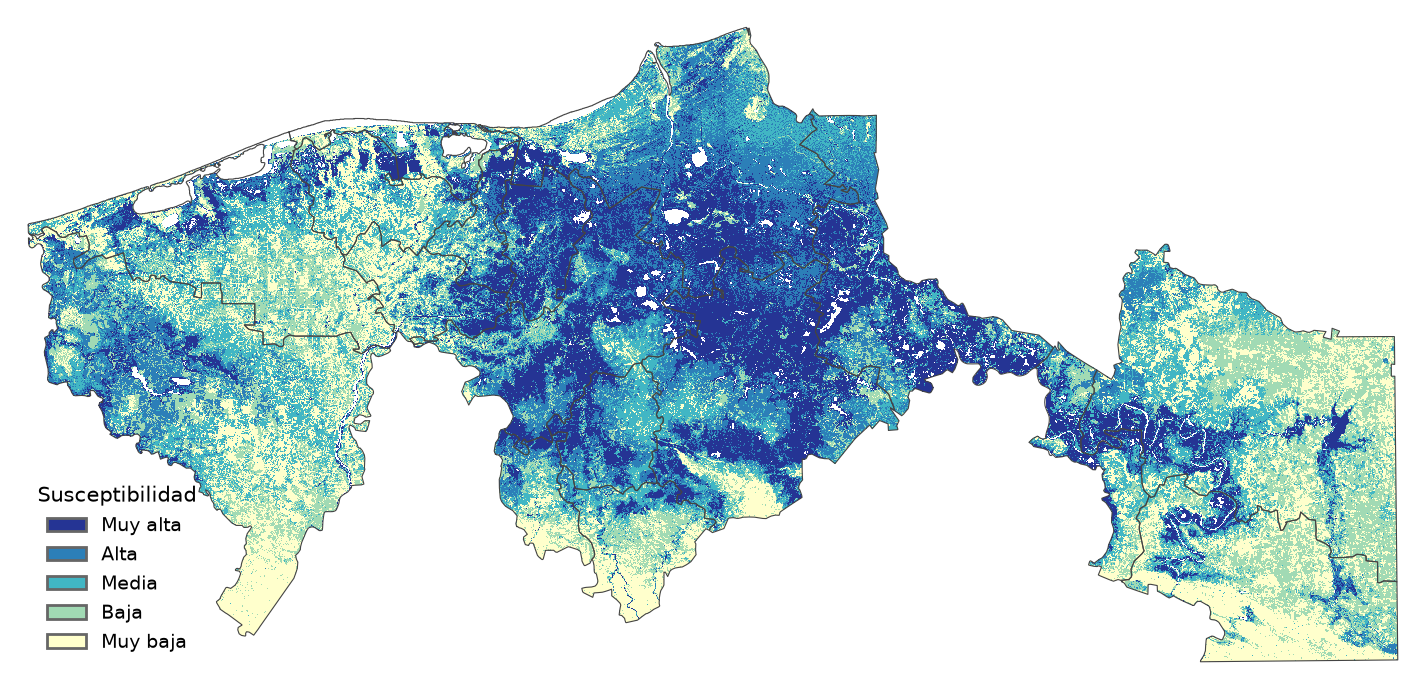
\includegraphics[width=0.95\textwidth]{figures/mapa_clases.png}\par
  \vspace{1.2cm}
  {\large Proyecto distributionMapApp\par}
  \vspace{0.2cm}
  {\normalsize Rama \texttt{feat/flood-risk-model} · octubre de 2026\par}
  \vfill
  {\small\color{gray} Fuentes: INEGI (LiDAR 5 m, CEM 3.0), CENAPRED, Copernicus Sentinel-1,
  JRC/CEMS GloFAS, MERIT Hydro, JRC Global Surface Water, ESA WorldCover, FAO GAUL 2025.\par}
\end{titlepage}

\tableofcontents
\newpage

\section*{Resumen}\addcontentsline{toc}{section}{Resumen}

Tabasco se inunda cada año y las inundaciones extremas, como las de 2007 y 2020, afectan a cientos de miles de personas. Este trabajo construye un mapa de susceptibilidad a inundación de todo el estado, a 30 m, solo con datos públicos y con un procedimiento reproducible, y lo valida contra inundaciones que los modelos no vieron durante el entrenamiento. Las variables de terreno se derivan del modelo digital de elevación LiDAR de 5 m de INEGI, acondicionado hidrológicamente a 15 m, e incluyen la altura sobre el drenaje más cercano (HAND). El mapa es un ensamble por promedio de rangos, con pesos iguales fijados a priori, de tres componentes: un modelo LightGBM entrenado con inundaciones extremas cartografiadas por CENAPRED (2011 y 2020), un modelo LightGBM entrenado con inundación estacional detectada con Sentinel-1 (2015--2025) y la profundidad de inundación de JRC/GloFAS para un periodo de retorno de 100 años. Sobre la inundación extrema de 2011, que ningún componente vio, el ensamble obtiene un ROC AUC de 0.778, frente a 0.766 de JRC. Sobre las temporadas 2023--2025, posteriores al mapa oficial IPCET-PNUD 2022, obtiene entre 0.715 y 0.723, frente a 0.608--0.624 del mapa oficial. Las clases Alta y Muy alta, que cubren el 40 \% del estado, concentran el 84 \% de la superficie inundada en 2011 y el 67 \% en 2023--2025, frente al 40 \% que concentraría un mapa aleatorio. El trabajo muestra también que la validación cruzada espacial (ROC 0.885) sobreestima la capacidad de anticipar inundaciones nuevas.

\textbf{Palabras clave:} susceptibilidad a inundación; LiDAR; HAND; Sentinel-1; LightGBM; ensamble; validación con eventos retenidos; Tabasco.

\section{Introducción}

Tabasco concentra cerca del 40 \% del agua dulce de México y recibe una precipitación media tres veces mayor que la nacional, con lluvias de mayo a noviembre {[}1{]}. El estado se inunda cada año; en 2020, los frentes fríos y los huracanes Gamma, Eta e Iota afectaron a unas 800 000 personas {[}1{]}. Para planear la prevención hace falta saber \textbf{dónde} es más probable que el agua llegue, antes de que ocurra el evento: un mapa de susceptibilidad.

El índice que usaba la aplicación de consulta de este proyecto (FHI) combinaba factores con reglas fijas. Sus valores se concentraban entre 18 y 64 de una escala 0--100 y nunca se había contrastado con inundaciones observadas. Este trabajo lo sustituye por un modelo aprendido de inundaciones reales y validado con eventos independientes.

\textbf{Pregunta de investigación.} ¿Es posible obtener, solo con datos públicos, un mapa de susceptibilidad a inundación de Tabasco que anticipe inundaciones futuras mejor que las referencias disponibles: la profundidad de inundación global de JRC, la elevación del terreno y el mapa oficial IPCET-PNUD 2022?

\textbf{Enfoque.}

\begin{enumerate}
\def\labelenumi{\arabic{enumi}.}
\tightlist
\item
  Aprender la susceptibilidad a partir de \textbf{inundaciones observadas}, en lugar de combinar factores con pesos fijados por criterio experto.
\item
  Usar el terreno más detallado disponible (\textbf{LiDAR de INEGI}) para describir la posición de cada celda respecto del drenaje.
\item
  Juzgar los modelos por su desempeño en \textbf{eventos retenidos}, es decir, inundaciones que ningún componente vio, y no solo por validación cruzada.
\end{enumerate}

\textbf{Definición del producto.} Es un \textbf{índice relativo de susceptibilidad}: ordena las celdas del estado según su propensión a inundarse. \textbf{No es una profundidad ni una probabilidad anual} (ver sección 5.1).

El resto del documento se organiza así. La sección 2 resume los trabajos relacionados. La sección 3 describe el área de estudio, los datos, el procesamiento del terreno, las etiquetas, los modelos y el protocolo de validación. La sección 4 presenta los resultados, la sección 5 los discute junto con las limitaciones, y la sección 6 presenta las conclusiones.

\section{Trabajos relacionados}

Los mapas de susceptibilidad a inundación con aprendizaje automático combinan variables del terreno, del suelo y de la hidrografía con un inventario de inundaciones pasadas. Tehrany et al.~{[}2{]} ensamblaron pesos de evidencia y máquinas de soporte vectorial para la cuenca de Terengganu, en Malasia. Khosravi et al.~{[}3{]} compararon cuatro algoritmos de árboles de decisión para inundaciones súbitas en la cuenca del Haraz, en Irán. En ambos casos, la evaluación principal es el área bajo la curva ROC sobre una partición aleatoria del inventario.

En Tabasco, los trabajos recientes usan imágenes satelitales para \textbf{cartografiar} el agua de un evento concreto. Pech-May et al.~{[}4{]} clasificaron cultivos y coberturas del oriente del estado con Sentinel-2 y SVM, RF y CART en Google Earth Engine. Con radar Sentinel-1 y la red U-Net, se segmentaron las inundaciones de 2020 en la subregión de los Ríos {[}1, 5{]}, se entrenó un modelo con el conjunto Sen1Floods11 aplicado al sureste de México {[}6{]} y se combinaron Sentinel-1 y Sentinel-2 entre 2019 y 2023 {[}7{]}.

\begin{longtable}[]{@{}
  >{\raggedright\arraybackslash}p{(\linewidth - 8\tabcolsep) * \real{0.2000}}
  >{\raggedright\arraybackslash}p{(\linewidth - 8\tabcolsep) * \real{0.2000}}
  >{\raggedright\arraybackslash}p{(\linewidth - 8\tabcolsep) * \real{0.2000}}
  >{\raggedright\arraybackslash}p{(\linewidth - 8\tabcolsep) * \real{0.2000}}
  >{\raggedright\arraybackslash}p{(\linewidth - 8\tabcolsep) * \real{0.2000}}@{}}
\caption{Trabajos relacionados: datos, modelo, área de estudio y producto.}\tabularnewline
\toprule\noalign{}
\begin{minipage}[b]{\linewidth}\raggedright
Trabajo
\end{minipage} & \begin{minipage}[b]{\linewidth}\raggedright
Datos
\end{minipage} & \begin{minipage}[b]{\linewidth}\raggedright
Modelo
\end{minipage} & \begin{minipage}[b]{\linewidth}\raggedright
Área de estudio
\end{minipage} & \begin{minipage}[b]{\linewidth}\raggedright
Producto
\end{minipage} \\
\midrule\noalign{}
\endfirsthead
\toprule\noalign{}
\begin{minipage}[b]{\linewidth}\raggedright
Trabajo
\end{minipage} & \begin{minipage}[b]{\linewidth}\raggedright
Datos
\end{minipage} & \begin{minipage}[b]{\linewidth}\raggedright
Modelo
\end{minipage} & \begin{minipage}[b]{\linewidth}\raggedright
Área de estudio
\end{minipage} & \begin{minipage}[b]{\linewidth}\raggedright
Producto
\end{minipage} \\
\midrule\noalign{}
\endhead
\bottomrule\noalign{}
\endlastfoot
Tehrany et al.~{[}2{]}, 2014 & Factores condicionantes en SIG e inventario & Pesos de evidencia + SVM & Terengganu, Malasia & Susceptibilidad \\
Khosravi et al.~{[}3{]}, 2018 & Factores condicionantes en SIG e inventario & LMT, REPT, NBT, ADT & Haraz, Irán & Susceptibilidad \\
Pech-May et al.~{[}4{]}, 2022 & Sentinel-2 & SVM, RF, CART & Oriente de Tabasco & Cobertura del suelo \\
Pech-May et al.~{[}1{]}, 2023 & Sentinel-1 (2020) & U-Net & Los Ríos, Tabasco & Mapa de un evento \\
Pech-May et al.~{[}6{]}, 2024 & Sentinel-1 (Sen1Floods11) & U-Net & Sureste de México & Mapa de un evento \\
Pech-May et al.~{[}7{]}, 2025 & Sentinel-1 y Sentinel-2 (2019--2023) & U-Net & Los Ríos, Tabasco & Mapa de un evento \\
Este trabajo & LiDAR, Sentinel-1, CENAPRED, JRC & LightGBM + ensamble & Todo Tabasco & Susceptibilidad \\
\end{longtable}

Este trabajo se diferencia en dos aspectos. Estima la susceptibilidad de todo el estado, no el agua de una imagen, y la valida con \textbf{eventos completos retenidos} en lugar de con una partición aleatoria de celdas, que mide sobre todo interpolación dentro de eventos conocidos {[}8{]}.

\section{Materiales y métodos}

\subsection{Área de estudio}

Tabasco ocupa 24 707 km² (área geodésica de los límites FAO GAUL 2025) y se divide en 17 municipios (figura 1). Casi todo el estado es una llanura baja formada por los ríos Grijalva y Usumacinta, que se unen antes de desembocar en el golfo de México. Solo el sur (la sierra, en Teapa, Tacotalpa y Huimanguillo) y algunas lomas del oriente superan unas decenas de metros de altitud. La temporada de lluvias va de mayo a noviembre, con máximos en junio y de septiembre a noviembre {[}1{]}.

\begin{figure}[H]\centering
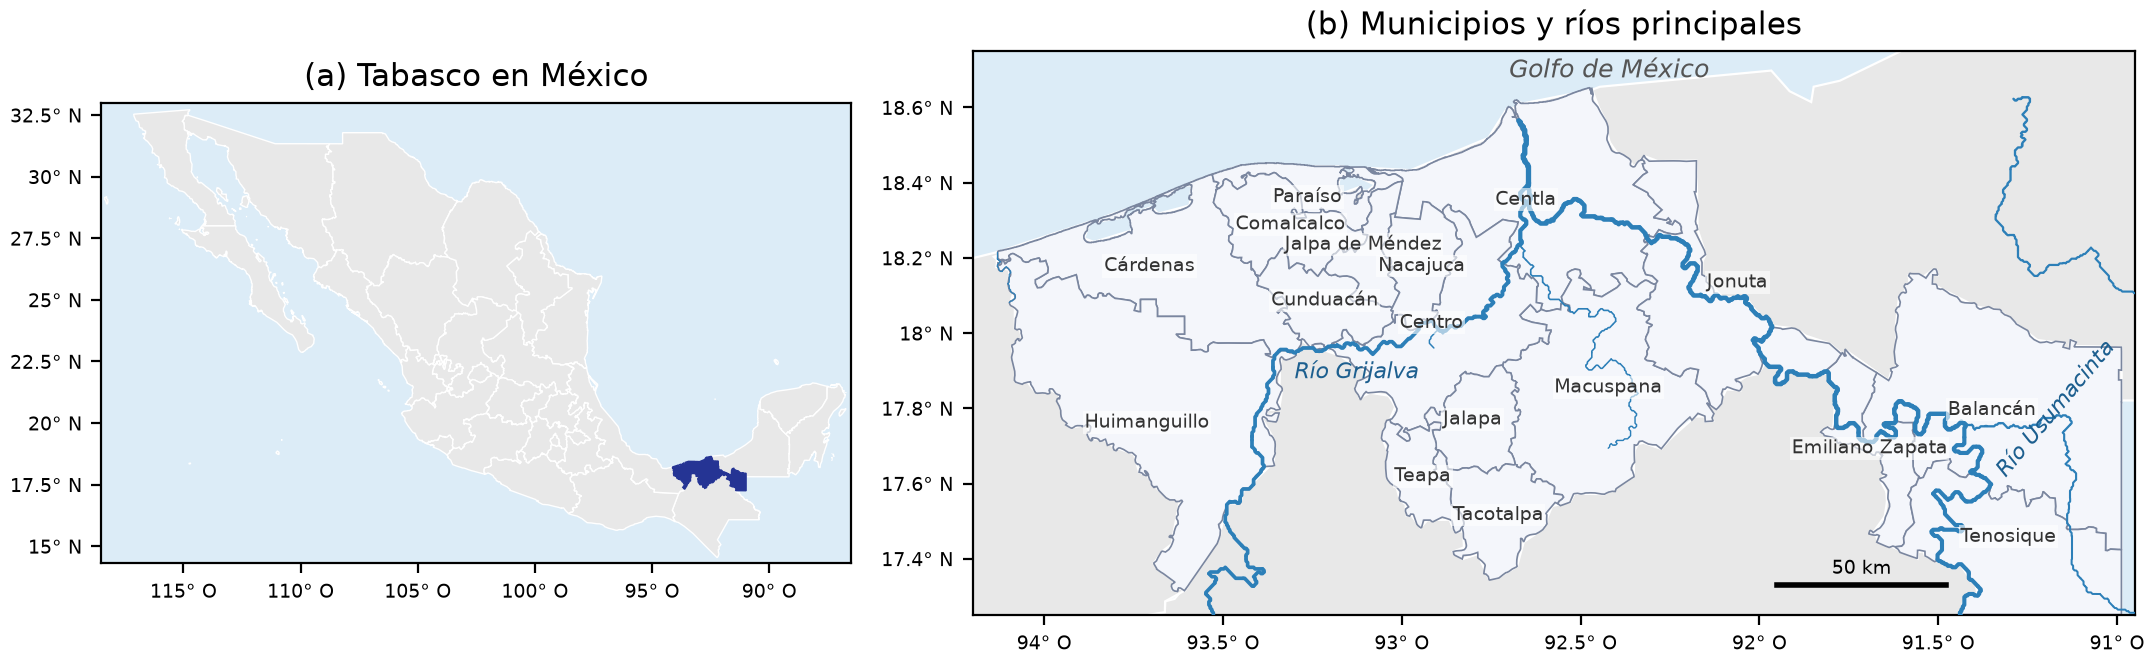
\includegraphics[width=\textwidth]{figures/area_estudio.png}
\caption{Área de estudio. (a) Tabasco en México; (b) municipios (FAO GAUL 2025) y ríos principales (HydroSHEDS).}
\end{figure}

\subsection{Datos}

\begin{longtable}[]{@{}
  >{\raggedright\arraybackslash}p{(\linewidth - 4\tabcolsep) * \real{0.3333}}
  >{\raggedright\arraybackslash}p{(\linewidth - 4\tabcolsep) * \real{0.3333}}
  >{\raggedright\arraybackslash}p{(\linewidth - 4\tabcolsep) * \real{0.3333}}@{}}
\caption{Fuentes de datos.}\tabularnewline
\toprule\noalign{}
\begin{minipage}[b]{\linewidth}\raggedright
Fuente
\end{minipage} & \begin{minipage}[b]{\linewidth}\raggedright
Uso
\end{minipage} & \begin{minipage}[b]{\linewidth}\raggedright
Resolución / periodo
\end{minipage} \\
\midrule\noalign{}
\endfirsthead
\toprule\noalign{}
\begin{minipage}[b]{\linewidth}\raggedright
Fuente
\end{minipage} & \begin{minipage}[b]{\linewidth}\raggedright
Uso
\end{minipage} & \begin{minipage}[b]{\linewidth}\raggedright
Resolución / periodo
\end{minipage} \\
\midrule\noalign{}
\endhead
\bottomrule\noalign{}
\endlastfoot
INEGI, MDE LiDAR (terreno) & Elevación, HAND, pendiente, TWI, acumulación de flujo & 5 m → 15 m; vuelo 2007, edición 2012; 603 hojas (1.6 GB); cubre el 85.6 \% de la tierra del estado \\
INEGI, Continuo de Elevaciones Mexicano 3.0 & Relleno de los huecos del LiDAR & 15 m; todo el estado; elevaciones en metros enteros \\
CENAPRED, Atlas Nacional de Riesgos & Etiquetas de eventos extremos: inundación del 22-oct-2011; 2020 (Cristóbal, Sentinel-1 28-oct y 5-nov, TerraSAR-X 7-nov, Copernicus) & Polígonos vectoriales \\
CENAPRED, mapas PNUD 2018 e IPCET-PNUD 2022 & \textbf{Solo comparación}, nunca entrenamiento & Polígonos, 5 clases \\
Copernicus Sentinel-1 GRD (VV) & Etiquetas de inundación estacional 2015--2025 & 10 m → 30 m \\
JRC/CEMS GloFAS Flood Hazard v2.1 {[}9{]} & Profundidad por periodo de retorno (10 y 100 años): variable y componente del ensamble & ≈ 90 m \\
MERIT Hydro {[}10{]} & Área de drenaje aguas arriba, HAND de referencia, último recurso de relleno & ≈ 90 m \\
JRC Global Surface Water v1.4 {[}11{]} & Exclusión de agua permanente (ocurrencia ≥ 50 \%) & 30 m \\
ESA WorldCover 2021 & Uso de suelo & 10 m \\
FAO GAUL 2025 nivel 2 & Límite estatal y 17 municipios & Vectorial \\
\end{longtable}

\textbf{Grilla de modelado:} UTM 15N (EPSG:32615), 30 m, 11 248 × 5 282 celdas (límite estatal + 2 km). Celdas etiquetadas dentro del estado: 23 742 km² (se excluye el agua permanente).

\subsection{Terreno: del LiDAR al HAND}

\subsubsection{Resolución: 10 m → 15 m}

La resolución prevista era 10 m. A esa escala, el relleno de depresiones por costo mínimo (\emph{least-cost breaching}) no es viable en un equipo de escritorio para todo el estado. Se trabajó a \textbf{15 m}, con el algoritmo híbrido de Lindsay {[}12{]}, que da redes de drenaje equivalentes a un costo mucho menor. Las variables se agregan después a la grilla de modelado de 30 m.

\subsubsection{Acondicionamiento hidrológico}

El LiDAR de INEGI \textbf{no tiene datos sobre ríos y lagunas} (el láser no vuelve del agua), deja huecos donde no hubo vuelo y guarda el mar como una superficie plana a 0.0 m. Si no se corrige, el HAND {[}13{]} (altura sobre el drenaje más cercano) queda referido a cauces equivocados.

\begin{enumerate}
\def\labelenumi{\arabic{enumi}.}
\tightlist
\item
  Los huecos se rellenan primero con el CEM 3.0 de INEGI (15 m) y, donde tampoco hay CEM, con MERIT (≈ 90 m). Cada fuente se corrige por su sesgo vertical mediano respecto del LiDAR: \textbf{−0.40 m} para el CEM y \textbf{−1.64 m} para MERIT.
\item
  El agua (ocurrencia JRC ≥ 50 \% o área de drenaje MERIT ≥ 500 km²) se incorpora a la red de drenaje.
\end{enumerate}

\subsubsection{Cálculo del HAND sin quemado de cauces}

Una práctica común es ``quemar'' los cauces, es decir, rebajar el MDE donde hay agua. En la costa de Tabasco esto falla: como el LiDAR guarda el mar como una superficie plana a 0.0 m, las lagunas quemadas 5 m quedaban \textbf{más bajas que su propia salida al mar}. El algoritmo de \emph{breaching} tallaba caminos larguísimos y el MDE llegaba a \textbf{−7 011 m}. El HAND resultante era absurdo: Centla daba 28 m de HAND a 1.4 m sobre el nivel del mar.

Por eso el MDE rellenado solo define las direcciones de flujo (D8). El HAND se mide sobre la elevación acondicionada, contra el primer cauce, cuerpo de agua o mar al que drena cada celda. Ese punto se obtiene etiquetando cuencas: cada salida lleva codificada su elevación. En un caso sintético (mar plano a 0 m y una laguna sin LiDAR) se verificó que se cumple la propiedad HAND ≤ elevación − mínima elevación de drenaje.

\subsubsection{Cobertura del estado}

Una primera versión del dominio dejaba dos huecos de cobertura, que se corrigieron antes de la evaluación final:

\begin{longtable}[]{@{}
  >{\raggedright\arraybackslash}p{(\linewidth - 4\tabcolsep) * \real{0.3333}}
  >{\raggedright\arraybackslash}p{(\linewidth - 4\tabcolsep) * \real{0.3333}}
  >{\raggedright\arraybackslash}p{(\linewidth - 4\tabcolsep) * \real{0.3333}}@{}}
\caption{Huecos de cobertura del dominio y su corrección.}\tabularnewline
\toprule\noalign{}
\begin{minipage}[b]{\linewidth}\raggedright
Problema
\end{minipage} & \begin{minipage}[b]{\linewidth}\raggedright
Magnitud
\end{minipage} & \begin{minipage}[b]{\linewidth}\raggedright
Corrección
\end{minipage} \\
\midrule\noalign{}
\endfirsthead
\toprule\noalign{}
\begin{minipage}[b]{\linewidth}\raggedright
Problema
\end{minipage} & \begin{minipage}[b]{\linewidth}\raggedright
Magnitud
\end{minipage} & \begin{minipage}[b]{\linewidth}\raggedright
Corrección
\end{minipage} \\
\midrule\noalign{}
\endhead
\bottomrule\noalign{}
\endlastfoot
La grilla seguía la extensión de las hojas LiDAR, no el límite estatal & 391 km² fuera del modelo: 332 km² de Huimanguillo (9 \%) y 59 km² de Cárdenas (3 \%), en la planicie del Tonalá & Grilla = límite estatal + 2 km \\
3 103 km² de tierra (12.6 \% del estado) sin LiDAR, rellenados con MERIT a ≈ 90 m & Paraíso 91 \%, Comalcalco 63 \%, Emiliano Zapata 44 \%, Tacotalpa 34 \%, Jalpa de Méndez 31 \% & Relleno con el CEM 3.0 de INEGI a 15 m, que cubre más del \textbf{97 \%} de los huecos; MERIT solo en el resto \\
\end{longtable}

Otras series de INEGI a 5 m y 1.5 m cubren solo el 21 \% del hueco y mezclan datum y vuelos, así que no se usaron. Tras la corrección no queda ninguna celda de tierra del estado sin clase. Al ampliar la grilla, la superficie sin LiDAR pasó a 3 416 km² (14.4 \% de la tierra del estado), porque la franja agregada al oeste tampoco tiene vuelo LiDAR.

Con la corrección, los porcentajes por clase de cada municipio cambiaron como máximo 2.6 puntos (Cárdenas), y la validación cambió en la tercera cifra decimal. El modelo se apoya sobre todo en JRC, la elevación y el uso de suelo, y la mediana del CEM difiere poco de la de MERIT (−1.3 m). Lo que mejora es el detalle local del terreno y la cobertura de la cuenca del Tonalá.

\subsection{Etiquetas}

\subsubsection{Eventos extremos (CENAPRED)}

\begin{itemize}
\tightlist
\item
  \textbf{Inundada (1):} la celda cae dentro de cualquier polígono de evento.
\item
  \textbf{Seca (0):} el resto del estado.
\item
  \textbf{Excluida:} el agua permanente y todo lo que queda fuera de Tabasco, porque CENAPRED solo mapeó dentro del estado.
\end{itemize}

Resultado: 14.9 \% de celdas inundadas.

\subsubsection{Fuentes adicionales evaluadas}

Con solo dos años de eventos extremos, los modelos generalizaban mal (sección 4.2). Se evaluaron fuentes adicionales contrastándolas con los polígonos de CENAPRED del mismo año, mediante la intersección sobre la unión (IoU), la precisión (P) y la exhaustividad (R):

\begin{longtable}[]{@{}
  >{\raggedright\arraybackslash}p{(\linewidth - 6\tabcolsep) * \real{0.2500}}
  >{\raggedright\arraybackslash}p{(\linewidth - 6\tabcolsep) * \real{0.2500}}
  >{\raggedright\arraybackslash}p{(\linewidth - 6\tabcolsep) * \real{0.2500}}
  >{\raggedright\arraybackslash}p{(\linewidth - 6\tabcolsep) * \real{0.2500}}@{}}
\caption{Fuentes de etiquetas evaluadas frente a los polígonos de CENAPRED del mismo año.}\tabularnewline
\toprule\noalign{}
\begin{minipage}[b]{\linewidth}\raggedright
Fuente
\end{minipage} & \begin{minipage}[b]{\linewidth}\raggedright
Método
\end{minipage} & \begin{minipage}[b]{\linewidth}\raggedright
Concordancia con CENAPRED
\end{minipage} & \begin{minipage}[b]{\linewidth}\raggedright
Decisión
\end{minipage} \\
\midrule\noalign{}
\endfirsthead
\toprule\noalign{}
\begin{minipage}[b]{\linewidth}\raggedright
Fuente
\end{minipage} & \begin{minipage}[b]{\linewidth}\raggedright
Método
\end{minipage} & \begin{minipage}[b]{\linewidth}\raggedright
Concordancia con CENAPRED
\end{minipage} & \begin{minipage}[b]{\linewidth}\raggedright
Decisión
\end{minipage} \\
\midrule\noalign{}
\endhead
\bottomrule\noalign{}
\endlastfoot
Landsat 5/7 (2011; 2007) & MNDWI \textgreater{} 0 en píxeles despejados (QA), sin agua permanente & 2011: IoU 7.7 \% (P 12.9 \%, R 16.1 \%); 2007: solo 6 \% del estado inundado & \textbf{Descartada:} las nubes ocultan el pico, y las imágenes despejadas son posteriores a la crecida \\
Global Flood Database (MODIS) {[}14{]} & Eventos 2005, 2007, 2010, 2011 & 2011: IoU 14.1 \% (P 17.7 \%, R 40.4 \%); vistas despejadas medianas: 1 \% & \textbf{Descartada} \\
Sentinel-1, detección por cambio & VV percentil 10 (jun--dic) \textless{} −13 dB \textbf{y} caída \textgreater{} 1.5 dB respecto de la mediana feb--may del mismo año, HAND MERIT \textless{} 20 m, sin agua permanente & 2020: \textbf{IoU 34.9 \%} (P 55.5 \%, R 48.5 \%) & \textbf{Adoptada} como etiqueta de inundación estacional \\
Sentinel-1, ``vegetación inundada'' (doble rebote) & Aumento de VV \textgreater{} 2 dB & Unión con la anterior: P 16.4 \%, R 71.7 \% & \textbf{Descartada:} demasiado ruido \\
\end{longtable}

Los umbrales de Sentinel-1 se calibraron con un barrido de 34 combinaciones contra los polígonos de 2020. Detectan sobre todo la \textbf{inundación estacional recurrente}: entre 470 y 1 092 km² por año en 2015--2025, sin un pico marcado en 2020. Por eso se tratan como un fenómeno distinto de los eventos extremos de CENAPRED (sección 4.3).

\subsection{Modelos}

Todos los modelos usan LightGBM {[}15{]} con los mismos hiperparámetros: 400 árboles, tasa de aprendizaje 0.05, 63 hojas, mínimo de 50 muestras por hoja y submuestreo de 0.8 en filas y columnas. Se entrena con un muestreo balanceado de 150 000 celdas por clase. Las variables son las 6 del terreno LiDAR agregado a 30 m más las capas JRC, MERIT y WorldCover.

\textbf{Fuga de etiquetas.} Las capas JRC Global Surface Water (ocurrencia y extensión máxima) pueden haber registrado las mismas inundaciones que se usan como etiqueta. Con ellas, la validación cruzada espacial da ROC 0.890; sin ellas, 0.885 ± 0.010. La diferencia es despreciable, así que se excluyeron para evitar la fuga.

\textbf{Ensamble.} El mapa final promedia los rangos de tres componentes: el modelo de eventos extremos, el modelo estacional y la profundidad JRC para 100 años. El rango de una celda es su función de distribución empírica sobre las celdas del estado, de modo que los tres componentes quedan en la misma escala 0--1. \textbf{Los pesos son iguales y se fijaron a priori}; no se ajustaron mirando los eventos de prueba. La sección 4.4 documenta cómo se llegó a esta combinación.

\textbf{Clases.} El índice se divide en quintiles de superficie: Muy baja, Baja, Media, Alta y Muy alta. Por construcción, cada clase cubre ≈ 20 \% del estado.

\subsection{Protocolo de validación y métricas}

La evaluación final reconstruye el ensamble con versiones de los componentes que \textbf{no vieron} los eventos de prueba:

\begin{longtable}[]{@{}lll@{}}
\caption{Protocolo de validación final: entrenamiento y prueba de cada componente.}\tabularnewline
\toprule\noalign{}
Componente & Entrenamiento & Prueba \\
\midrule\noalign{}
\endfirsthead
\toprule\noalign{}
Componente & Entrenamiento & Prueba \\
\midrule\noalign{}
\endhead
\bottomrule\noalign{}
\endlastfoot
Extremos & CENAPRED 2020 (5 capas) & CENAPRED 2011 \\
Estacional & S1 2015--2022 & S1 2023, 2024, 2025 \\
Referencias & JRC 100 años, elevación, IPCET-PNUD 2022 & Los mismos eventos \\
\end{longtable}

Muestra de evaluación: 1 000 000 de celdas válidas (semilla fija). El mapa publicado usa, en cambio, modelos entrenados con \textbf{todos} los eventos.

Se usan tres métricas, todas calculadas sobre la muestra de evaluación:

\begin{itemize}
\tightlist
\item
  \textbf{ROC AUC.} Probabilidad de que una celda inundada elegida al azar reciba un índice mayor que una celda seca elegida al azar. Un mapa aleatorio obtiene 0.5.
\item
  \textbf{PR AUC} (precisión promedio). Resume la precisión a lo largo de todos los umbrales. Es sensible a la rareza de la inundación: un mapa aleatorio obtiene la tasa base, es decir, la proporción de celdas inundadas.
\item
  \textbf{Captura en Alta + Muy alta.} Proporción de las celdas inundadas en el evento que caen en las dos clases más altas, es decir, en el 40 \% del estado con mayor índice. Es la exhaustividad (\emph{recall}) del mapa de clases. Un mapa aleatorio captura el 40 \%.
\end{itemize}

Este trabajo no reporta precisión, exhaustividad ni F1 a un umbral libre, que son las métricas habituales para \textbf{cartografiar} el agua de una imagen {[}1{]}. Un mapa de susceptibilidad no tiene un umbral natural: sus clases se definen por superficie. Al corte de Alta + Muy alta, la precisión queda acotada por la rareza del evento (como máximo, la tasa base dividida entre 0.4, es decir, ≈ 11 \% para 2011), así que F1 mediría más la extensión del evento que la calidad del mapa. ROC y PR AUC evalúan el orden completo, y la captura evalúa el corte que efectivamente se publica.

\section{Resultados}

\subsection{Validación física del HAND}

El HAND no usó las inundaciones de CENAPRED, así que esos polígonos sirven para validarlo:

\begin{longtable}[]{@{}lll@{}}
\caption{HAND dentro y fuera de las manchas de inundación de CENAPRED.}\tabularnewline
\toprule\noalign{}
Evento & HAND mediano dentro / fuera de la mancha & Celdas inundadas con HAND ≤ 5 m \\
\midrule\noalign{}
\endfirsthead
\toprule\noalign{}
Evento & HAND mediano dentro / fuera de la mancha & Celdas inundadas con HAND ≤ 5 m \\
\midrule\noalign{}
\endhead
\bottomrule\noalign{}
\endlastfoot
Cristóbal 2020 & 0.30 m / 2.0 m & 99.8 \% \\
22-oct-2011 & 0.45 m / 2.0 m & 97.7 \% \\
\end{longtable}

Solo un 0.42 \% de las celdas no encuentra drenaje, y ninguna supera su propia elevación.

\subsection{La validación cruzada espacial sobreestima}

\begin{quote}
Las cifras de las secciones 4.2 a 4.4 son de los experimentos de exploración, hechos antes de la corrección de cobertura (sección 3.3.4). La evaluación definitiva, ya con la cobertura corregida, está en la sección 4.5. Las diferencias aparecen en la tercera cifra decimal.
\end{quote}

Con bloques espaciales de 5 km (\emph{StratifiedGroupKFold}, 5 pliegues), el modelo de eventos extremos logra ROC 0.885 ± 0.010, PR 0.871 (muestra balanceada) y Brier 0.136, frente a ROC 0.740 de la mejor variable sola (JRC 100 años).

Pero al \textbf{entrenar solo con 2020 y evaluar en 2011}:

\begin{longtable}[]{@{}lll@{}}
\caption{Modelo entrenado con 2020 y evaluado en 2011, frente a variables solas.}\tabularnewline
\toprule\noalign{}
Índice & ROC & PR (tasa base 0.046) \\
\midrule\noalign{}
\endfirsthead
\toprule\noalign{}
Índice & ROC & PR (tasa base 0.046) \\
\midrule\noalign{}
\endhead
\bottomrule\noalign{}
\endlastfoot
Modelo (2020 → 2011) & 0.741 & 0.091 \\
JRC 100 años & 0.759 & 0.090 \\
Elevación & 0.758 & 0.092 \\
\end{longtable}

\textbf{Diagnóstico.} Las manchas de inundación miden decenas de kilómetros, así que bloques de 5 km no logran descorrelacionarlas {[}8{]}. La validación cruzada espacial mide sobre todo interpolación dentro de eventos conocidos. Además, solo el 28 \% de la superficie inundada en 2011 se volvió a inundar en 2020: los eventos son muy distintos entre sí.

\textbf{Comparación justa con el mapa oficial.} Sobre los eventos de CENAPRED, IPCET-PNUD 2022 obtiene ROC 0.892 en 2011 y 0.848 en 2020, y PNUD 2018 obtiene 0.768 y 0.783. Como IPCET es de 2022, esa comparación no es justa. Por eso se definió como prueba justa \textbf{las temporadas de Sentinel-1 de 2023 a 2025}, posteriores a IPCET y a los datos de entrenamiento del modelo. Con esa prueba, el modelo de eventos extremos ya supera a IPCET en PR AUC todos los años; por ejemplo, a 90 m: 0.114 contra 0.087 en 2023, 0.076 contra 0.058 en 2024 y 0.112 contra 0.088 en 2025.

\subsection{Variantes de etiqueta y el sesgo del detector}

Evaluación sobre Sentinel-1 2023--2025, a 30 m, con la media de ROC / PR:

\begin{longtable}[]{@{}llll@{}}
\caption{Variantes de etiqueta: media de ROC / PR en Sentinel-1 2023--2025 y ROC en CENAPRED 2011.}\tabularnewline
\toprule\noalign{}
Variante & Etiquetas de entrenamiento & S1 2023--25 & CENAPRED 2011 (independiente) \\
\midrule\noalign{}
\endfirsthead
\toprule\noalign{}
Variante & Etiquetas de entrenamiento & S1 2023--25 & CENAPRED 2011 (independiente) \\
\midrule\noalign{}
\endhead
\bottomrule\noalign{}
\endlastfoot
a & CENAPRED (2011 + 2020) & 0.637 / 0.196 & (lo vio) \\
a′ & CENAPRED 2020 & --- & 0.749 \\
b & CENAPRED + S1 2015--2022 & 0.753 / 0.281 & (lo vio) \\
b′ & CENAPRED 2020 + S1 2015--2022 & 0.758 / 0.284 & 0.707 \\
c & Solo S1 2015--2022 & 0.769 / 0.304 & \textbf{0.694} \\
--- & JRC 100 años & 0.575 / 0.149 & 0.767 \\
--- & IPCET-PNUD 2022 & 0.614 / 0.170 & (probablemente lo vio) \\
\end{longtable}

Las variantes entrenadas con Sentinel-1 ganan con claridad sobre etiquetas de Sentinel-1, pero \textbf{pierden contra JRC sobre un evento extremo independiente} (c: 0.694 contra 0.767). Se entrenan y evalúan con el mismo detector, así que aprenden también sus errores sistemáticos, y la prueba los premia. Hay dos ``mundos'' de etiqueta con fenómenos distintos: eventos extremos (CENAPRED) e inundación estacional (Sentinel-1). Ningún modelo único gana en ambos.

\subsection{Selección del ensamble}

ROC / PR de cada combinación, con componentes que no vieron los eventos de prueba:

\begin{longtable}[]{@{}
  >{\raggedright\arraybackslash}p{(\linewidth - 8\tabcolsep) * \real{0.2000}}
  >{\raggedright\arraybackslash}p{(\linewidth - 8\tabcolsep) * \real{0.2000}}
  >{\raggedright\arraybackslash}p{(\linewidth - 8\tabcolsep) * \real{0.2000}}
  >{\raggedright\arraybackslash}p{(\linewidth - 8\tabcolsep) * \real{0.2000}}
  >{\raggedright\arraybackslash}p{(\linewidth - 8\tabcolsep) * \real{0.2000}}@{}}
\caption{ROC / PR de cada combinación de componentes.}\tabularnewline
\toprule\noalign{}
\begin{minipage}[b]{\linewidth}\raggedright
Combinación
\end{minipage} & \begin{minipage}[b]{\linewidth}\raggedright
CENAPRED 2011
\end{minipage} & \begin{minipage}[b]{\linewidth}\raggedright
S1 2023
\end{minipage} & \begin{minipage}[b]{\linewidth}\raggedright
S1 2024
\end{minipage} & \begin{minipage}[b]{\linewidth}\raggedright
S1 2025
\end{minipage} \\
\midrule\noalign{}
\endfirsthead
\toprule\noalign{}
\begin{minipage}[b]{\linewidth}\raggedright
Combinación
\end{minipage} & \begin{minipage}[b]{\linewidth}\raggedright
CENAPRED 2011
\end{minipage} & \begin{minipage}[b]{\linewidth}\raggedright
S1 2023
\end{minipage} & \begin{minipage}[b]{\linewidth}\raggedright
S1 2024
\end{minipage} & \begin{minipage}[b]{\linewidth}\raggedright
S1 2025
\end{minipage} \\
\midrule\noalign{}
\endhead
\bottomrule\noalign{}
\endlastfoot
Modelo extremos (2020) & 0.741 / 0.091 & 0.668 / 0.253 & 0.669 / 0.185 & 0.676 / 0.272 \\
Modelo estacional (S1) & 0.690 / 0.078 & 0.783 / 0.387 & 0.782 / 0.333 & 0.771 / 0.379 \\
JRC & 0.761 / 0.091 & 0.591 / 0.197 & 0.608 / 0.144 & 0.597 / 0.202 \\
0.5 extremos + 0.5 estacional & 0.742 / 0.092 & 0.748 / 0.336 & 0.746 / 0.275 & 0.746 / 0.345 \\
\textbf{extremos + estacional + JRC (1/3 c/u)} & \textbf{0.784 / 0.108} & 0.720 / 0.305 & 0.724 / 0.236 & 0.721 / 0.312 \\
\end{longtable}

El ensamble de tres componentes es el único que \textbf{supera a JRC en el evento extremo no visto} y conserva una ventaja amplia en la inundación estacional. Se adoptó como producto.

\subsection{Validación final con eventos retenidos}

La tabla 10 resume la evaluación con el protocolo de la sección 3.6. El ensamble es el único mapa que supera a todas las referencias en la inundación extrema no vista (2011), excepto a IPCET, que probablemente la usó. En las temporadas posteriores a 2022, que ningún mapa vio, el ensamble supera a JRC y a IPCET por unos 0.10--0.15 de ROC AUC y por un 33--67 \% relativo en PR AUC (59--67 \% frente a JRC, 33--56 \% frente a IPCET).

\begin{longtable}[]{@{}
  >{\raggedright\arraybackslash}p{(\linewidth - 8\tabcolsep) * \real{0.2000}}
  >{\raggedright\arraybackslash}p{(\linewidth - 8\tabcolsep) * \real{0.2000}}
  >{\raggedright\arraybackslash}p{(\linewidth - 8\tabcolsep) * \real{0.2000}}
  >{\raggedright\arraybackslash}p{(\linewidth - 8\tabcolsep) * \real{0.2000}}
  >{\raggedright\arraybackslash}p{(\linewidth - 8\tabcolsep) * \real{0.2000}}@{}}
\caption{ROC AUC / PR AUC sobre eventos retenidos. * El mapa IPCET-PNUD 2022 es posterior a 2011 y probablemente se calibró con esa inundación, así que para él 2011 no es un evento ``no visto''. Las temporadas 2023--2025 sí son posteriores a su publicación.}\tabularnewline
\toprule\noalign{}
\begin{minipage}[b]{\linewidth}\raggedright
Mapa
\end{minipage} & \begin{minipage}[b]{\linewidth}\raggedright
CENAPRED 2011 (evento extremo) ROC / PR
\end{minipage} & \begin{minipage}[b]{\linewidth}\raggedright
S1 2023 ROC / PR
\end{minipage} & \begin{minipage}[b]{\linewidth}\raggedright
S1 2024 ROC / PR
\end{minipage} & \begin{minipage}[b]{\linewidth}\raggedright
S1 2025 ROC / PR
\end{minipage} \\
\midrule\noalign{}
\endfirsthead
\toprule\noalign{}
\begin{minipage}[b]{\linewidth}\raggedright
Mapa
\end{minipage} & \begin{minipage}[b]{\linewidth}\raggedright
CENAPRED 2011 (evento extremo) ROC / PR
\end{minipage} & \begin{minipage}[b]{\linewidth}\raggedright
S1 2023 ROC / PR
\end{minipage} & \begin{minipage}[b]{\linewidth}\raggedright
S1 2024 ROC / PR
\end{minipage} & \begin{minipage}[b]{\linewidth}\raggedright
S1 2025 ROC / PR
\end{minipage} \\
\midrule\noalign{}
\endhead
\bottomrule\noalign{}
\endlastfoot
\textbf{Ensamble (este trabajo)} & \textbf{0.778 / 0.109} & \textbf{0.723 / 0.271} & \textbf{0.715 / 0.179} & \textbf{0.723 / 0.275} \\
Profundidad JRC 100 años & 0.766 / 0.091 & 0.569 / 0.168 & 0.576 / 0.108 & 0.577 / 0.173 \\
Elevación (más baja = más susceptible) & 0.751 / 0.085 & 0.568 / 0.177 & 0.557 / 0.111 & 0.587 / 0.188 \\
IPCET-PNUD 2022 (mapa oficial, 5 clases) & 0.892* / 0.200* & 0.609 / 0.188 & 0.608 / 0.115 & 0.624 / 0.207 \\
Tasa base (proporción inundada) & 0.045 & 0.139 & 0.084 & 0.144 \\
\end{longtable}

\begin{figure}[H]\centering
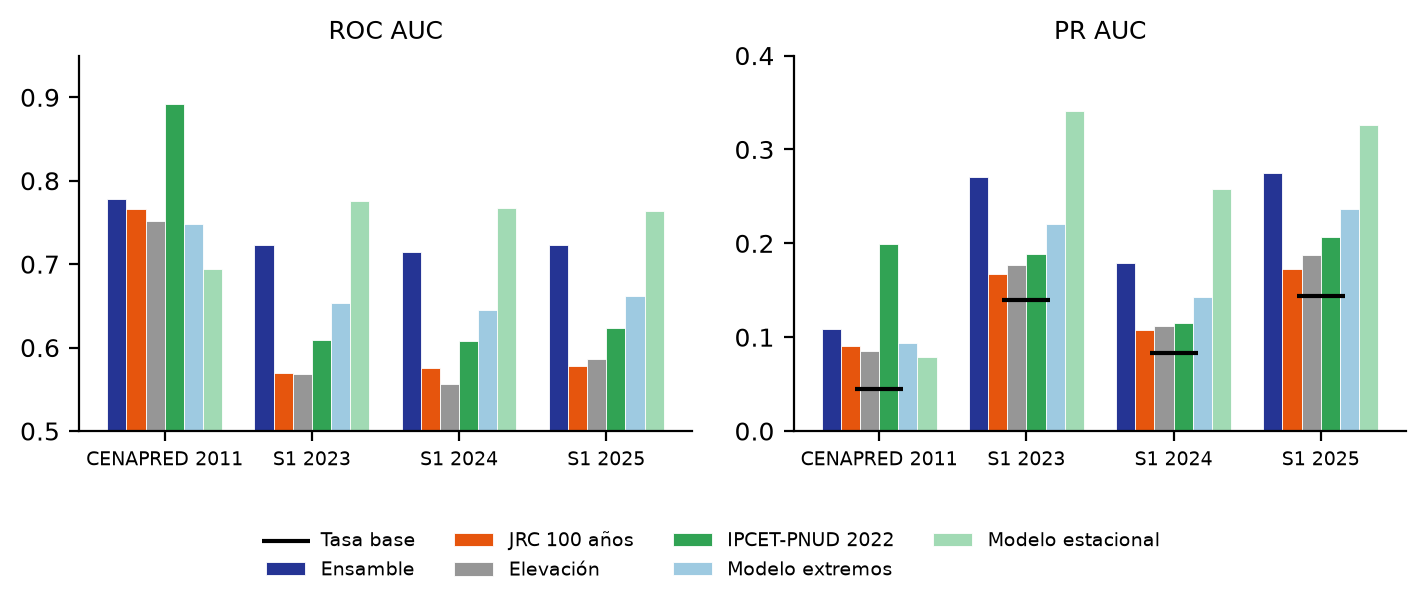
\includegraphics[width=\textwidth]{figures/validacion.png}
\caption{ROC AUC y PR AUC sobre eventos no vistos por los componentes del ensamble. La línea negra en PR AUC es la tasa base (proporción inundada).}
\end{figure}

La tabla 11 evalúa el corte que se publica: la captura en las clases Alta y Muy alta. En las temporadas 2023--2025, el ensamble concentra el 67 \% de la superficie inundada en el 40 \% del estado, frente a 51--53 \% de JRC y 46--50 \% de la elevación. En 2011 concentra el 84 \%, algo por debajo de JRC (87 \%): el ensamble ordena mejor el evento en conjunto (mayor ROC y PR AUC), pero JRC deja menos celdas inundadas en las tres clases bajas. IPCET no es directamente comparable, porque sus cinco clases hacen que el corte equivalente abarque el 57 \% del estado. En 2023--2025 captura el 70--71 \%, de 13 a 14 puntos más que un mapa aleatorio de esa superficie; el ensamble supera al azar por 27 puntos.

\begin{longtable}[]{@{}llllll@{}}
\caption{Captura en Alta + Muy alta: proporción de la superficie inundada de cada evento que cae en las clases altas de cada mapa. «Superficie» es la proporción del estado que cubren esas clases; un mapa aleatorio captura esa misma proporción. * IPCET probablemente vio el evento de 2011.}\tabularnewline
\toprule\noalign{}
Mapa & Superficie & CENAPRED 2011 & S1 2023 & S1 2024 & S1 2025 \\
\midrule\noalign{}
\endfirsthead
\toprule\noalign{}
Mapa & Superficie & CENAPRED 2011 & S1 2023 & S1 2024 & S1 2025 \\
\midrule\noalign{}
\endhead
\bottomrule\noalign{}
\endlastfoot
\textbf{Ensamble} & 40 \% & 84 \% & \textbf{67 \%} & \textbf{67 \%} & \textbf{67 \%} \\
JRC 100 años & 40 \% & \textbf{87 \%} & 51 \% & 53 \% & 52 \% \\
Elevación & 40 \% & 78 \% & 47 \% & 46 \% & 50 \% \\
IPCET-PNUD 2022 & 57 \% & 99 \%* & 70 \% & 70 \% & 71 \% \\
\end{longtable}

Los modelos publicados, entrenados con todos los eventos, obtienen en validación cruzada espacial ROC 0.884 ± 0.005 (eventos extremos) y 0.821 ± 0.006 (estacional). Las variables con mayor ganancia son, en el primero, JRC 100 años (31.1 \%), la elevación (22.0 \%), WorldCover (14.6 \%) y el área de drenaje (12.5 \%); en el segundo, \textbf{WorldCover (54.2 \%)}, el HAND de MERIT (8.1 \%) y JRC 10 años (6.5 \%).

\subsection{Mapa de susceptibilidad}

\begin{figure}[H]\centering
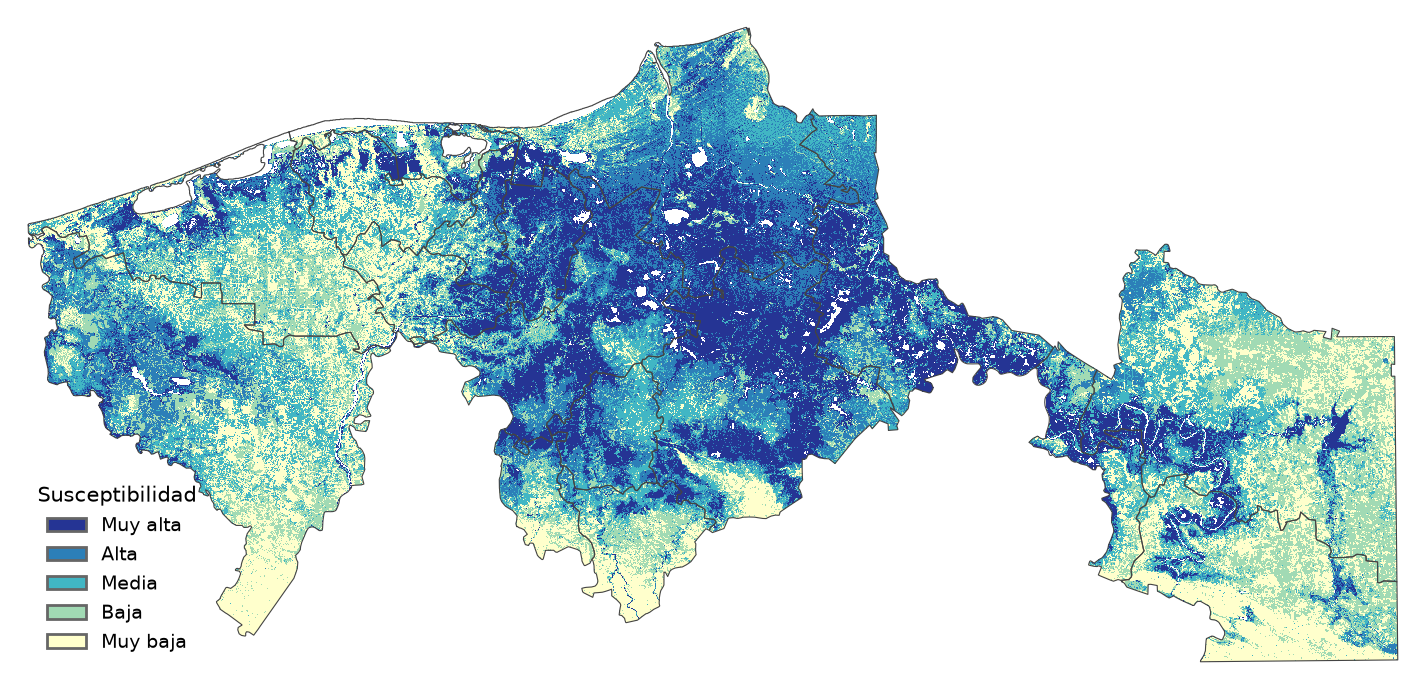
\includegraphics[width=\textwidth]{figures/mapa_clases.png}
\caption{Mapa de susceptibilidad: clases (quintiles de superficie del estado) y límites municipales (FAO GAUL 2025).}
\end{figure}

Los cortes de los quintiles del índice son 0.344, 0.474, 0.597 y 0.749. La susceptibilidad muy alta se concentra en la llanura baja del Grijalva y el Usumacinta. La sierra del sur y las lomas del oriente quedan en las clases bajas. La tabla 12 ordena los municipios por el puntaje medio del índice e indica el porcentaje de su superficie en clase Alta o Muy alta.

\begin{longtable}[]{@{}llll@{}}
\caption{Municipios por puntaje medio del índice. El orden sigue el puntaje medio, no el porcentaje. Las áreas excluyen el agua permanente.}\tabularnewline
\toprule\noalign{}
\# & Municipio & km² & \% Alta + Muy alta \\
\midrule\noalign{}
\endfirsthead
\toprule\noalign{}
\# & Municipio & km² & \% Alta + Muy alta \\
\midrule\noalign{}
\endhead
\bottomrule\noalign{}
\endlastfoot
1 & Nacajuca & 522 & 84 \% \\
2 & Jonuta & 1 520 & 71 \% \\
3 & Centro & 1 654 & 73 \% \\
4 & Macuspana & 2 348 & 71 \% \\
5 & Centla & 2 531 & 68 \% \\
6 & Jalapa & 593 & 57 \% \\
7 & Jalpa de Méndez & 366 & 55 \% \\
8 & Emiliano Zapata & 560 & 36 \% \\
9 & Paraíso & 321 & 33 \% \\
10 & Cunduacán & 592 & 30 \% \\
11 & Comalcalco & 743 & 21 \% \\
12 & Teapa & 420 & 27 \% \\
13 & Cárdenas & 1 820 & 20 \% \\
14 & Huimanguillo & 3 654 & 23 \% \\
15 & Balancán & 3 520 & 17 \% \\
16 & Tacotalpa & 732 & 15 \% \\
17 & Tenosique & 1 844 & 10 \% \\
\end{longtable}

\subsection{Aplicación del resultado}

El mapa se integró como capa interactiva de consulta: muestra la clase y el municipio bajo el cursor, una ficha por municipio y una vista por municipio.

\begin{figure}[H]\centering
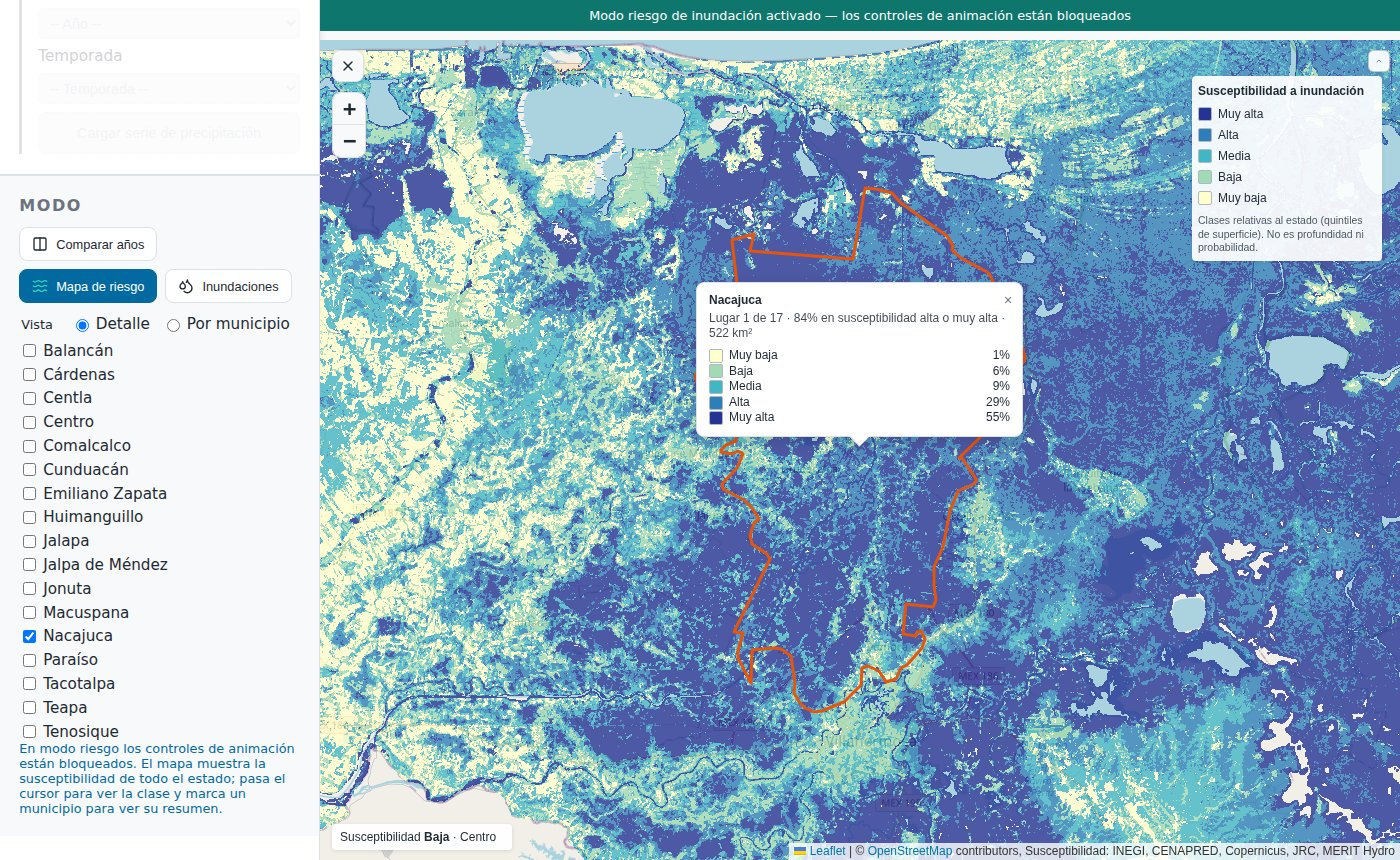
\includegraphics[width=\textwidth]{figures/app_detalle.jpg}
\caption{Consulta interactiva del mapa: capa estatal a 30 m, ficha de Nacajuca y lectura de la clase bajo el cursor.}
\end{figure}

\begin{figure}[H]\centering
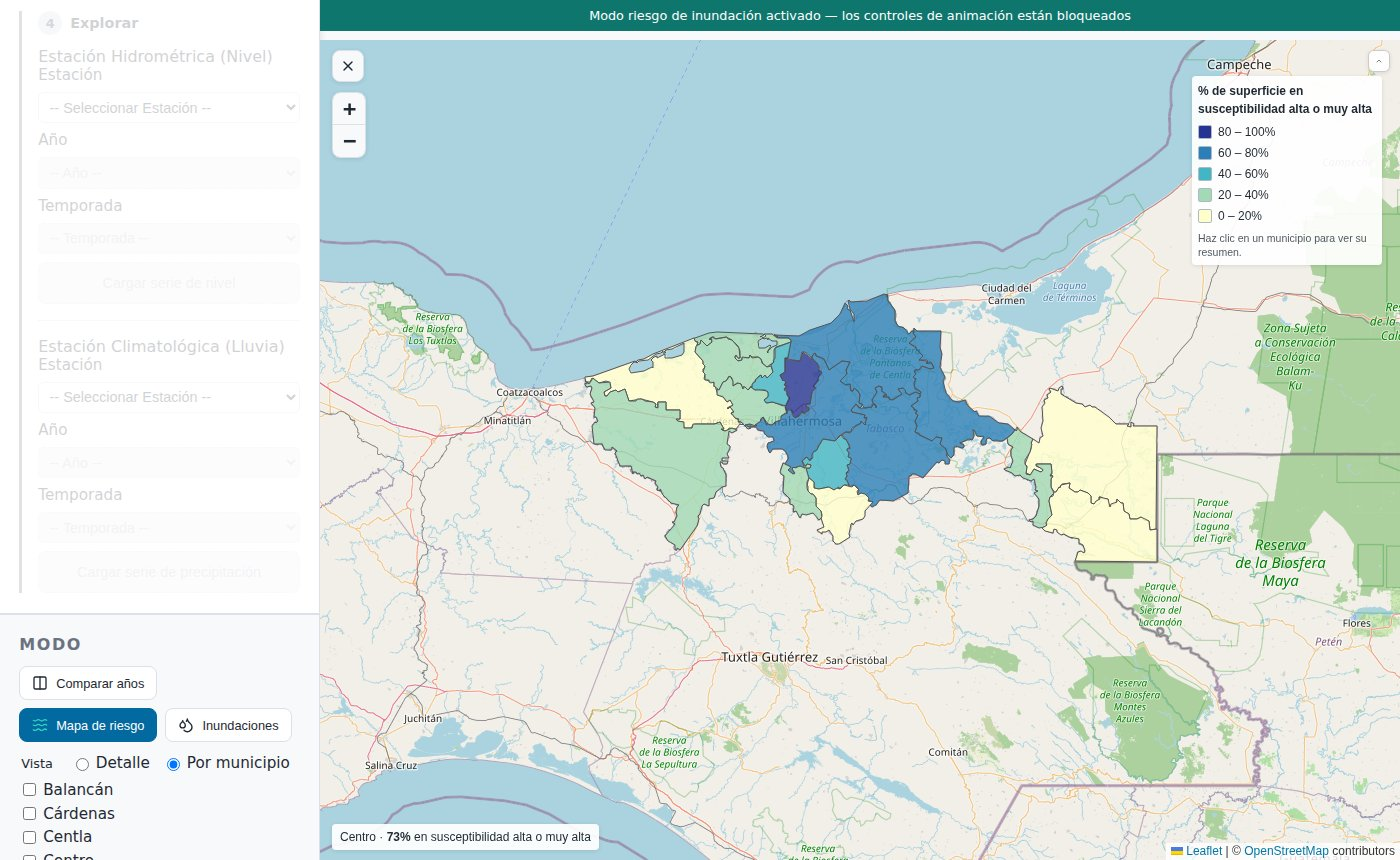
\includegraphics[width=\textwidth]{figures/app_municipios.jpg}
\caption{Vista por municipio: porcentaje de superficie en susceptibilidad alta o muy alta.}
\end{figure}

\section{Discusión}

El resultado principal es que un mapa aprendido de inundaciones observadas anticipa eventos nuevos mejor que las referencias disponibles, pero por un margen menor del que sugiere la validación cruzada. Frente a JRC, la ventaja en el evento extremo de 2011 es pequeña (0.778 contra 0.766) y no se sostiene en el corte publicado: JRC deja algo más de esa inundación en las clases altas (87 \% contra 84 \%). Frente a la elevación sola, la ventaja en ROC AUC es de 0.027. En la inundación estacional posterior a 2022 la ventaja es clara (0.10--0.15 de ROC AUC), aunque en parte la explica el sesgo compartido del detector (sección 5.1). El mapa oficial IPCET-PNUD 2022 es la referencia más fuerte en 2011, pero no se puede juzgar con ese evento; en los años que no vio, queda por debajo del ensamble.

La lección metodológica es que \textbf{la forma de validar decide la conclusión}. Con validación cruzada espacial, el modelo de eventos extremos parecía muy superior a JRC (0.885 contra 0.740). Al retener un evento completo, la ventaja desaparece (0.741 contra 0.759). Los estudios de susceptibilidad que validan con particiones aleatorias del inventario {[}2, 3{]} miden, por tanto, una capacidad distinta de la que importa para la prevención.

Los trabajos de cartografía de inundaciones con U-Net en Tabasco {[}1, 5--7{]} resuelven un problema complementario. Su F1 (por ejemplo, 0.93 para la clase inundación en {[}1{]}) mide la concordancia con la máscara de referencia de la misma imagen; las métricas de este trabajo miden qué tan bien un mapa previo ordena un evento futuro. Los dos números no son comparables. La relación natural entre ambos enfoques es otra: las máscaras de una U-Net son una fuente de \textbf{etiquetas} más limpias que el detector por umbrales usado aquí, cuya concordancia con CENAPRED es de 34.9 \% de IoU.

\subsection{Limitaciones y amenazas a la validez}

\begin{enumerate}
\def\labelenumi{\arabic{enumi}.}
\tightlist
\item
  \textbf{Ruido de etiquetas.} Mapas independientes del mismo evento coinciden con IoU de 14--35 \%. Los AUC absolutos (≈ 0.7--0.78) están acotados por ese ruido. Las \textbf{comparaciones} entre mapas son más confiables que los valores absolutos.
\item
  \textbf{Sesgo compartido del detector Sentinel-1.} El modelo estacional y la prueba 2023--2025 comparten el mismo detector, lo que favorece al ensamble frente a IPCET y JRC en esa prueba. Por eso el criterio de adopción exigió además superar a JRC en un evento extremo independiente (2011).
\item
  \textbf{Dominio del uso de suelo en el modelo estacional (54 \% de la ganancia).} Puede reflejar un patrón real (humedales y pastizales inundables) o un artefacto del detector (por ejemplo, cultivos cosechados que se oscurecen en el radar). No se resolvió.
\item
  \textbf{Selección del ensamble.} Los pesos se fijaron a priori, pero la \emph{idea} de ensamblar surgió después de ver los resultados en 2011 y en 2023--2025. Hay cierto riesgo de sesgo de selección; la confirmación definitiva exige un evento futuro.
\item
  \textbf{Antigüedad del LiDAR (vuelo 2007).} Las obras de protección posteriores (bordos y el Plan Integral Hídrico de Tabasco tras 2007) no están en el MDE. Zonas protegidas de Villahermosa pueden aparecer más susceptibles de lo que son.
\item
  \textbf{Resolución y fuentes de terreno.} El terreno se procesó a 15 m, no a 10 m (sección 3.3.1). En el 14.4 \% de la tierra del estado sin LiDAR (3 416 km², incluida la franja agregada al oeste) el terreno sale del CEM 3.0, que tiene elevaciones en metros enteros y otra fecha de captura. Algunas variables (JRC y MERIT, ≈ 90 m) son más gruesas que la grilla.
\item
  \textbf{Clases relativas.} Los quintiles hacen que ≈ 40 \% del estado sea ``Alta'' o ``Muy alta'' por definición. El mapa ordena; no dice cuánto se inunda ni con qué frecuencia.
\item
  \textbf{Artefactos visibles.} Hay un rayado diagonal tenue en Centla, probablemente por las franjas de órbita de Sentinel-1.
\item
  \textbf{Límites.} La simplificación de GAUL dejó líneas sueltas en 3 municipios; se corrigió, y el efecto fue de 5 de 26.9 M celdas.
\end{enumerate}

\section{Conclusiones}

Solo con datos públicos es posible construir un mapa de susceptibilidad a inundación de todo Tabasco que anticipa eventos no vistos mejor que la profundidad global de JRC, la elevación y, en los años posteriores a su publicación, el mapa oficial IPCET-PNUD 2022. El mapa combina el terreno LiDAR de INEGI, dos modelos LightGBM entrenados con inundaciones extremas y estacionales, y JRC, en un ensamble con pesos fijados a priori.

El hallazgo más importante es metodológico. La validación cruzada espacial sobreestima la capacidad de anticipar inundaciones nuevas, y las etiquetas de un mismo detector premian a los modelos entrenados con él. Por eso este trabajo evalúa con eventos completos retenidos y exige que el mapa supere a JRC también en un evento extremo independiente. Con ese criterio, las ventajas son reales pero moderadas, y los valores absolutos están acotados por el ruido de las etiquetas.

Como trabajo futuro, la mejora con mayor impacto esperado es reemplazar el detector por umbrales de Sentinel-1 por una segmentación con U-Net, en la línea de {[}1, 5--7{]}, para obtener etiquetas estacionales menos ruidosas, incluida la vegetación inundada. También se proponen: incorporar más eventos extremos independientes (activaciones de Copernicus EMS y UNOSAT); incorporar el inventario de bordos y obras de protección de CONAGUA para corregir la sobreestimación en zonas protegidas; usar umbrales del detector por cobertura de suelo; validar por cuenca o con bloques de al menos 50 km; y calibrar el índice con regresión isotónica sobre eventos retenidos, para pasar de un orden relativo a una probabilidad interpretable.

\section*{Contribuciones de los autores}\addcontentsline{toc}{section}{Contribuciones de los autores}

Conceptualización, G.A.J.C. y F.P.-M.; metodología, software, análisis formal, visualización y redacción del borrador original, G.A.J.C.; supervisión y redacción (revisión y edición), F.P.-M.

\section*{Disponibilidad de datos y código}\addcontentsline{toc}{section}{Disponibilidad de datos y código}

Todas las fuentes de la sección 3.2 son públicas. El procedimiento completo, desde la descarga del LiDAR hasta el mapa final, está automatizado y versionado junto con la aplicación, y regenera cada resultado desde las fuentes. Se verificó la reproducibilidad de las etiquetas de Sentinel-1: regenerarlas desde Earth Engine con el procedimiento final dio las 11 temporadas (2015--2025) idénticas byte a byte a las usadas para calibrar los umbrales.

\section*{Conflictos de interés}\addcontentsline{toc}{section}{Conflictos de interés}

Los autores declaran no tener conflictos de interés.

\section*{Referencias}\addcontentsline{toc}{section}{Referencias}

\begin{enumerate}
\def\labelenumi{\arabic{enumi}.}
\tightlist
\item
  Pech-May, F.; Aquino-Santos, R.; Delgadillo-Partida, J. Sentinel-1 SAR images and deep learning for water body mapping. \emph{Remote Sensing} \textbf{2023}, 15, 3009. \url{https://doi.org/10.3390/rs15123009}
\item
  Tehrany, M. S.; Pradhan, B.; Jebur, M. N. Flood susceptibility mapping using a novel ensemble weights-of-evidence and support vector machine models in GIS. \emph{Journal of Hydrology} \textbf{2014}, 512, 332--343. \url{https://doi.org/10.1016/j.jhydrol.2014.03.008}
\item
  Khosravi, K.; Pham, B. T.; Chapi, K.; Shirzadi, A.; Shahabi, H.; Revhaug, I.; Prakash, I.; Bui, D. T. A comparative assessment of decision trees algorithms for flash flood susceptibility modeling at Haraz watershed, northern Iran. \emph{Science of the Total Environment} \textbf{2018}, 627, 744--755. \url{https://doi.org/10.1016/j.scitotenv.2018.01.266}
\item
  Pech-May, F.; Aquino-Santos, R.; Rios-Toledo, G.; Posadas-Durán, J. P. F. Mapping of land cover with optical images, supervised algorithms, and Google Earth Engine. \emph{Sensors} \textbf{2022}, 22, 4729. \url{https://doi.org/10.3390/s22134729}
\item
  Pech-May, F.; Sánchez-Hernández, J. V.; López-Gómez, L. A.; Magaña-Govea, J.; Mil-Chontal, E. M. Flooded areas detection through SAR images and U-NET deep learning model. \emph{Computación y Sistemas} \textbf{2023}, 27, 449--458. \url{https://doi.org/10.13053/cys-27-2-4624}
\item
  Pech-May, F.; Aquino-Santos, R.; Álvarez-Cárdenas, O.; Lozoya Arandia, J.; Ríos-Toledo, G. Segmentation and visualization of flooded areas through Sentinel-1 images and U-Net. \emph{IEEE Journal of Selected Topics in Applied Earth Observations and Remote Sensing} \textbf{2024}, 17, 8996--9008. \url{https://doi.org/10.1109/JSTARS.2024.3387452}
\item
  Pech-May, F.; Álvarez-Cárdenas, O.; Ríos-Toledo, G. Flood mapping through Sentinel-1, Sentinel-2 imagery and U-NET deep learning model. \emph{Computación y Sistemas} \textbf{2025}, 29, 393--407. \url{https://doi.org/10.13053/cys-29-1-5539}
\item
  Roberts, D. R. et al.~Cross-validation strategies for data with temporal, spatial, hierarchical, or phylogenetic structure. \emph{Ecography} \textbf{2017}, 40, 913--929.
\item
  European Commission, Joint Research Centre. CEMS GloFAS Flood Hazard maps v2.1. Conjunto de datos \texttt{JRC/CEMS\_GLOFAS/FloodHazard/v2\_1} en Google Earth Engine.
\item
  Yamazaki, D. et al.~MERIT Hydro: a high-resolution global hydrography map. \emph{Water Resources Research} \textbf{2019}, 55, 5053--5073.
\item
  Pekel, J.-F. et al.~High-resolution mapping of global surface water and its long-term changes. \emph{Nature} \textbf{2016}, 540, 418--422.
\item
  Lindsay, J. B. Efficient hybrid breaching-filling sink removal methods for flow path enforcement in digital elevation models. \emph{Hydrological Processes} \textbf{2016}, 30, 846--857.
\item
  Nobre, A. D. et al.~Height Above the Nearest Drainage -- a hydrologically relevant new terrain model. \emph{Journal of Hydrology} \textbf{2011}, 404, 13--29.
\item
  Tellman, B. et al.~Satellite imaging reveals increased proportion of population exposed to floods. \emph{Nature} \textbf{2021}, 596, 80--86.
\item
  Ke, G. et al.~LightGBM: A highly efficient gradient boosting decision tree. \emph{Advances in Neural Information Processing Systems} \textbf{2017}, 30.
\end{enumerate}

Fuentes de datos: INEGI, Modelo Digital de Elevación de alta resolución LiDAR (5 m) y Continuo de Elevaciones Mexicano 3.0 (15 m); CENAPRED, Atlas Nacional de Riesgos; Copernicus Sentinel-1; ESA WorldCover 2021; FAO GAUL 2025.


\end{document}
